\documentclass{article}
\usepackage[utf8]{inputenc}
\usepackage{geometry}
 \geometry{
 a4paper,
 total={170mm,257mm},
 left=20mm,
 top=20mm,
 }
 \usepackage{graphicx}
 \usepackage{subcaption}
 \usepackage{titling}
 \usepackage{float}

 \title{ASSIGNMENT 2: Computer Vision 792}
\author{Madhia Shabih}
\date{August 2024}
 
 \usepackage{fancyhdr}
\fancypagestyle{plain}{%  the preset of fancyhdr 
    \fancyhf{} % clear all header and footer fields
    \fancyfoot[L]{\thedate}
    \fancyhead[L]{24397644}
    \fancyhead[R]{\theauthor}
}
\makeatletter
\def\@maketitle{%
  \newpage
  \null
  \vskip 1em%
  \begin{center}%
  \let \footnote \thanks
    {\LARGE \@title \par}%
    \vskip 1em%
    %{\large \@date}%
  \end{center}%
  \par
  \vskip 1em}
\makeatother

\usepackage{lipsum}  
\usepackage{cmbright}

\begin{document}
\maketitle
\section{Question 1}
\begin{figure}[H]
    \centering
    \begin{subfigure}{.3\textwidth}
        \centering
        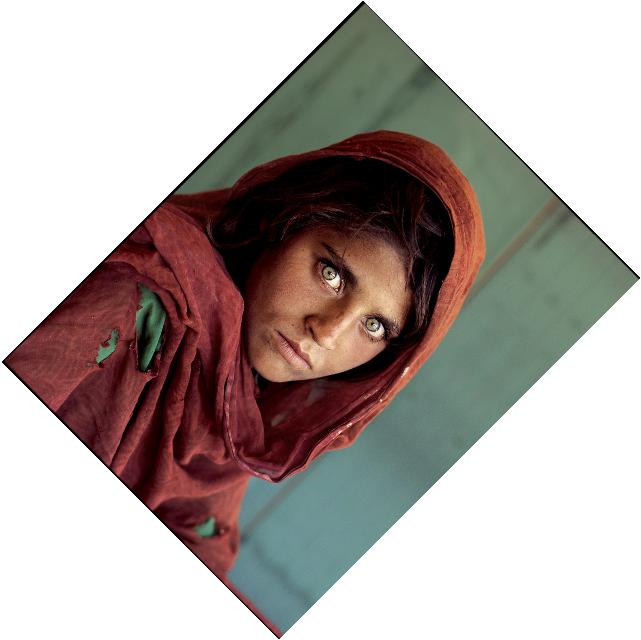
\includegraphics[scale=0.04]{q1/output/similar_0.5_0.5_2.jpg}
        \subcaption{}
    \end{subfigure}
    \begin{subfigure}{.3\textwidth}
        \centering
        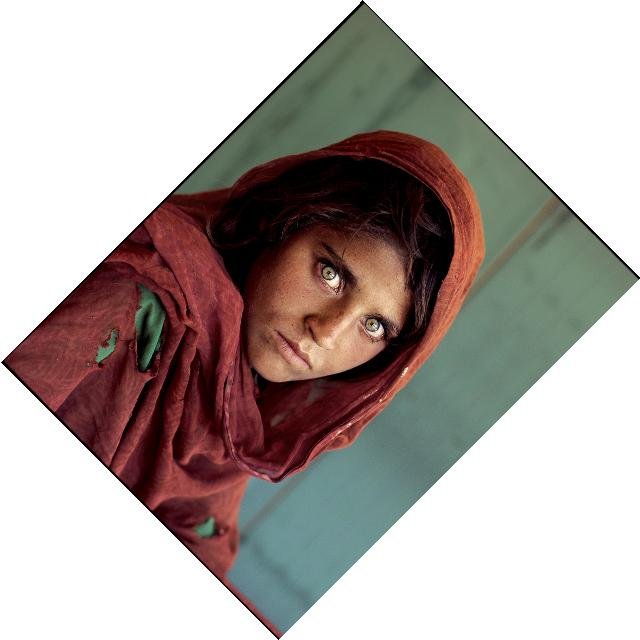
\includegraphics[scale=0.04]{q1/output/similar_0.5_1_2.jpg}
        \subcaption{}
    \end{subfigure}
    \begin{subfigure}{.3\textwidth}
        \centering
        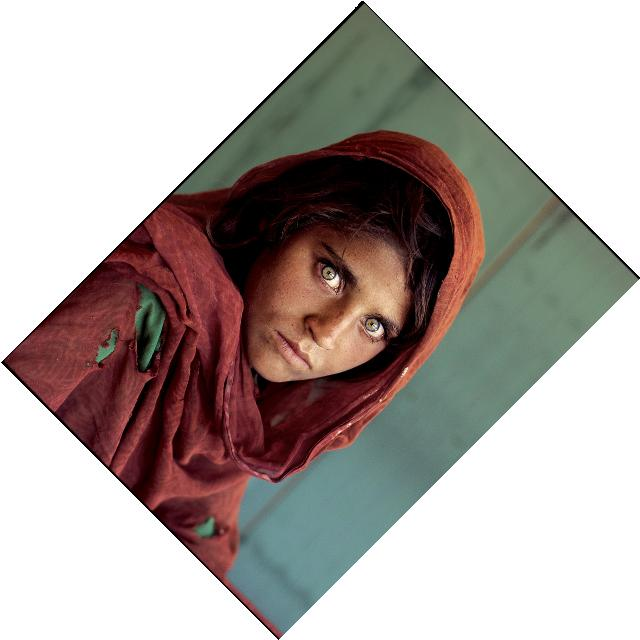
\includegraphics[scale=0.04]{q1/output/similar_0.5_2_2.jpg}
        \subcaption{}
    \end{subfigure}
    \caption{(a) blah (b) blah (c) blah}
\end{figure}

\begin{figure}[H]
    \centering
    \begin{subfigure}{.3\textwidth}
        \centering
        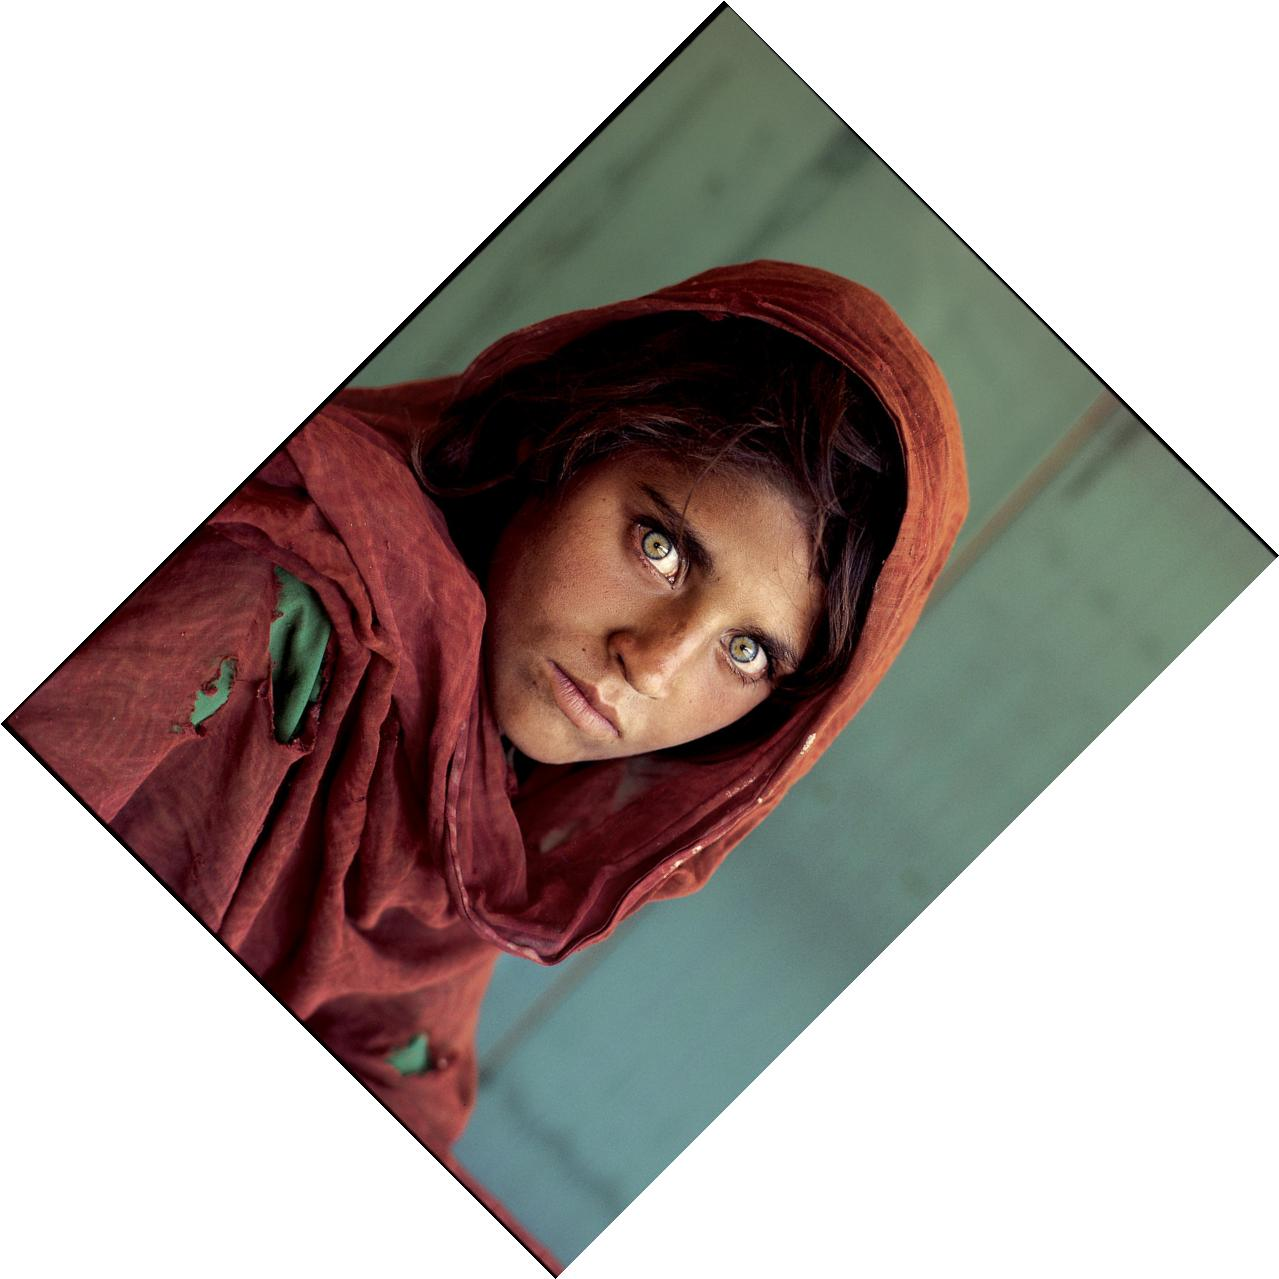
\includegraphics[scale=0.04]{q1/output/similar_1_0.5_2.jpg}
        \subcaption{}
    \end{subfigure}
    \begin{subfigure}{.3\textwidth}
        \centering
        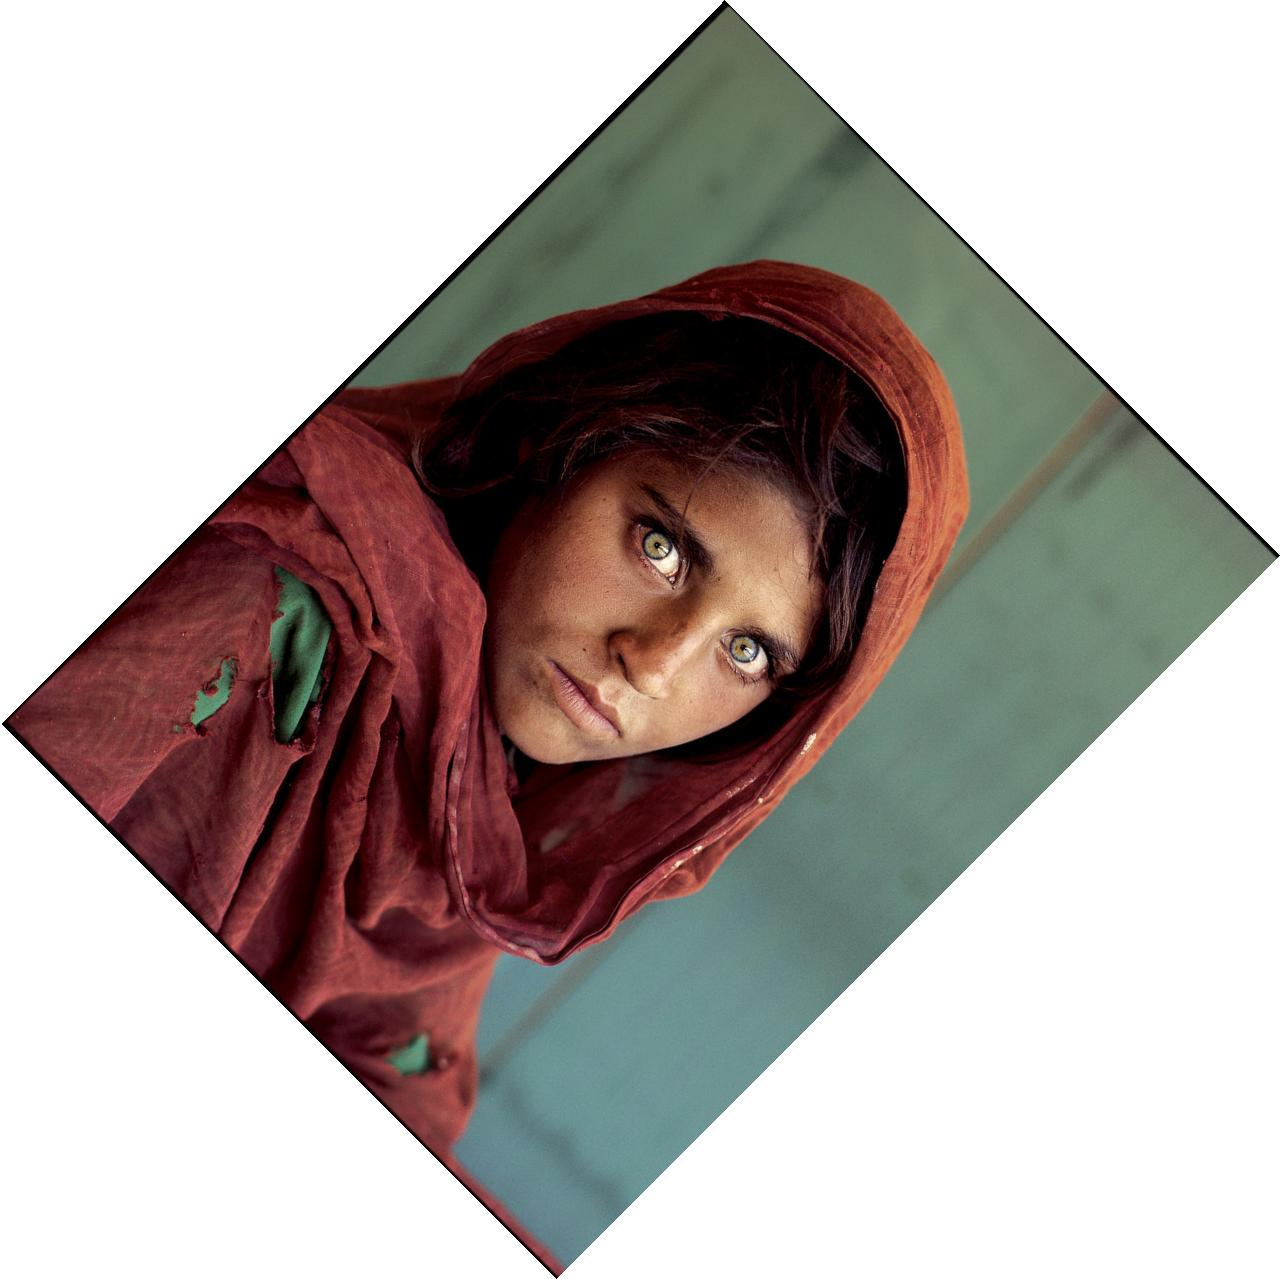
\includegraphics[scale=0.04]{q1/output/similar_1_1_2.jpg}
        \subcaption{}
    \end{subfigure}
    \begin{subfigure}{.3\textwidth}
        \centering
        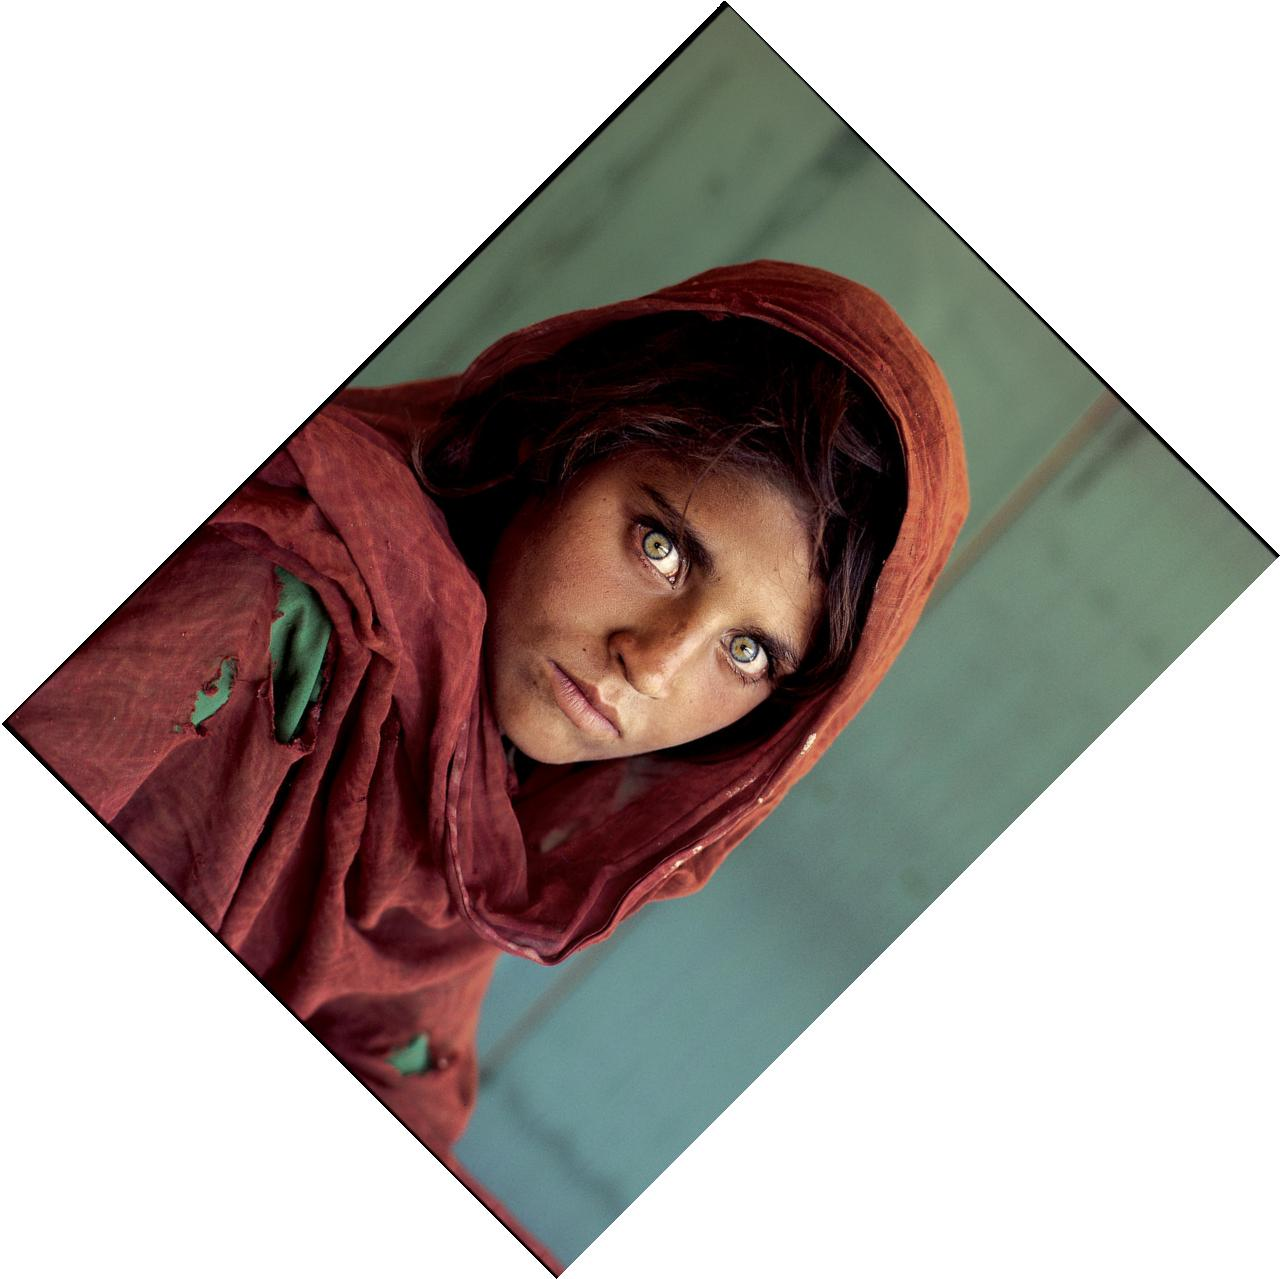
\includegraphics[scale=0.04]{q1/output/similar_1_2_2.jpg}
        \subcaption{}
    \end{subfigure}
    \caption{(a) blah (b) blah (c) blah}
\end{figure}

\begin{figure}[H]
    \centering
    \begin{subfigure}{.3\textwidth}
        \centering
        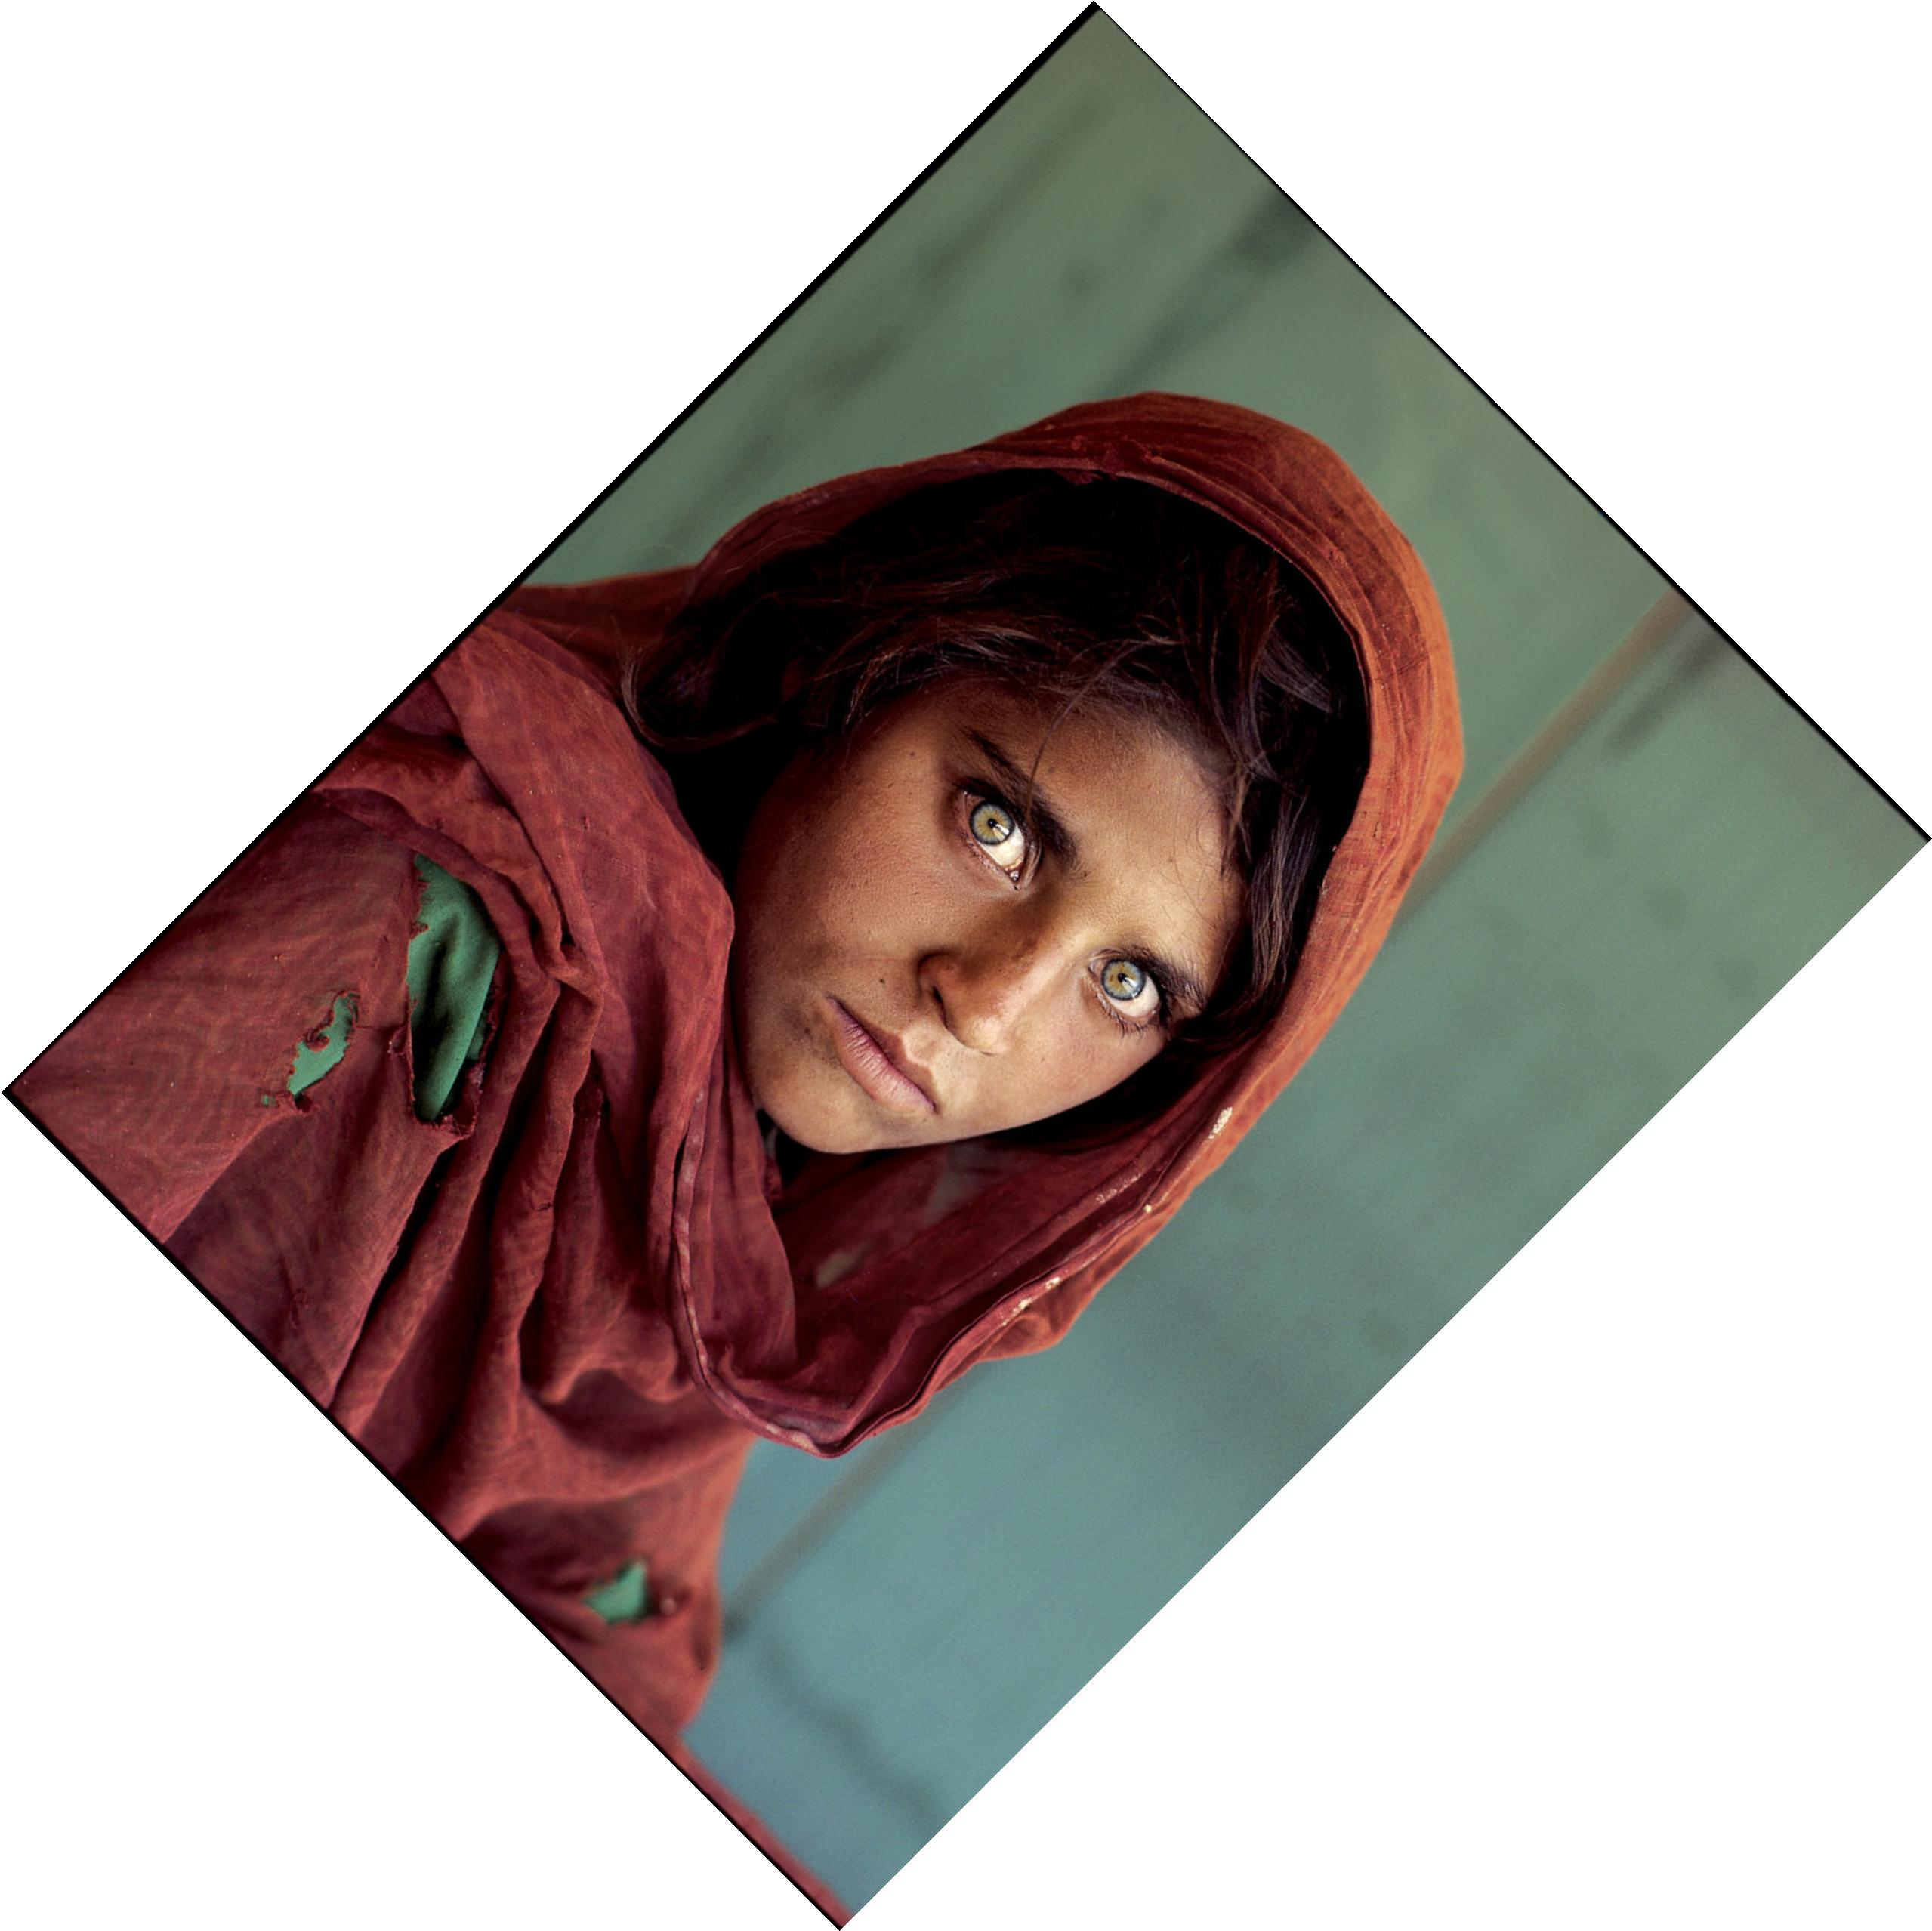
\includegraphics[scale=0.04]{q1/output/similar_2_0.5_2.jpg}
        \subcaption{}
    \end{subfigure}
    \begin{subfigure}{.3\textwidth}
        \centering
        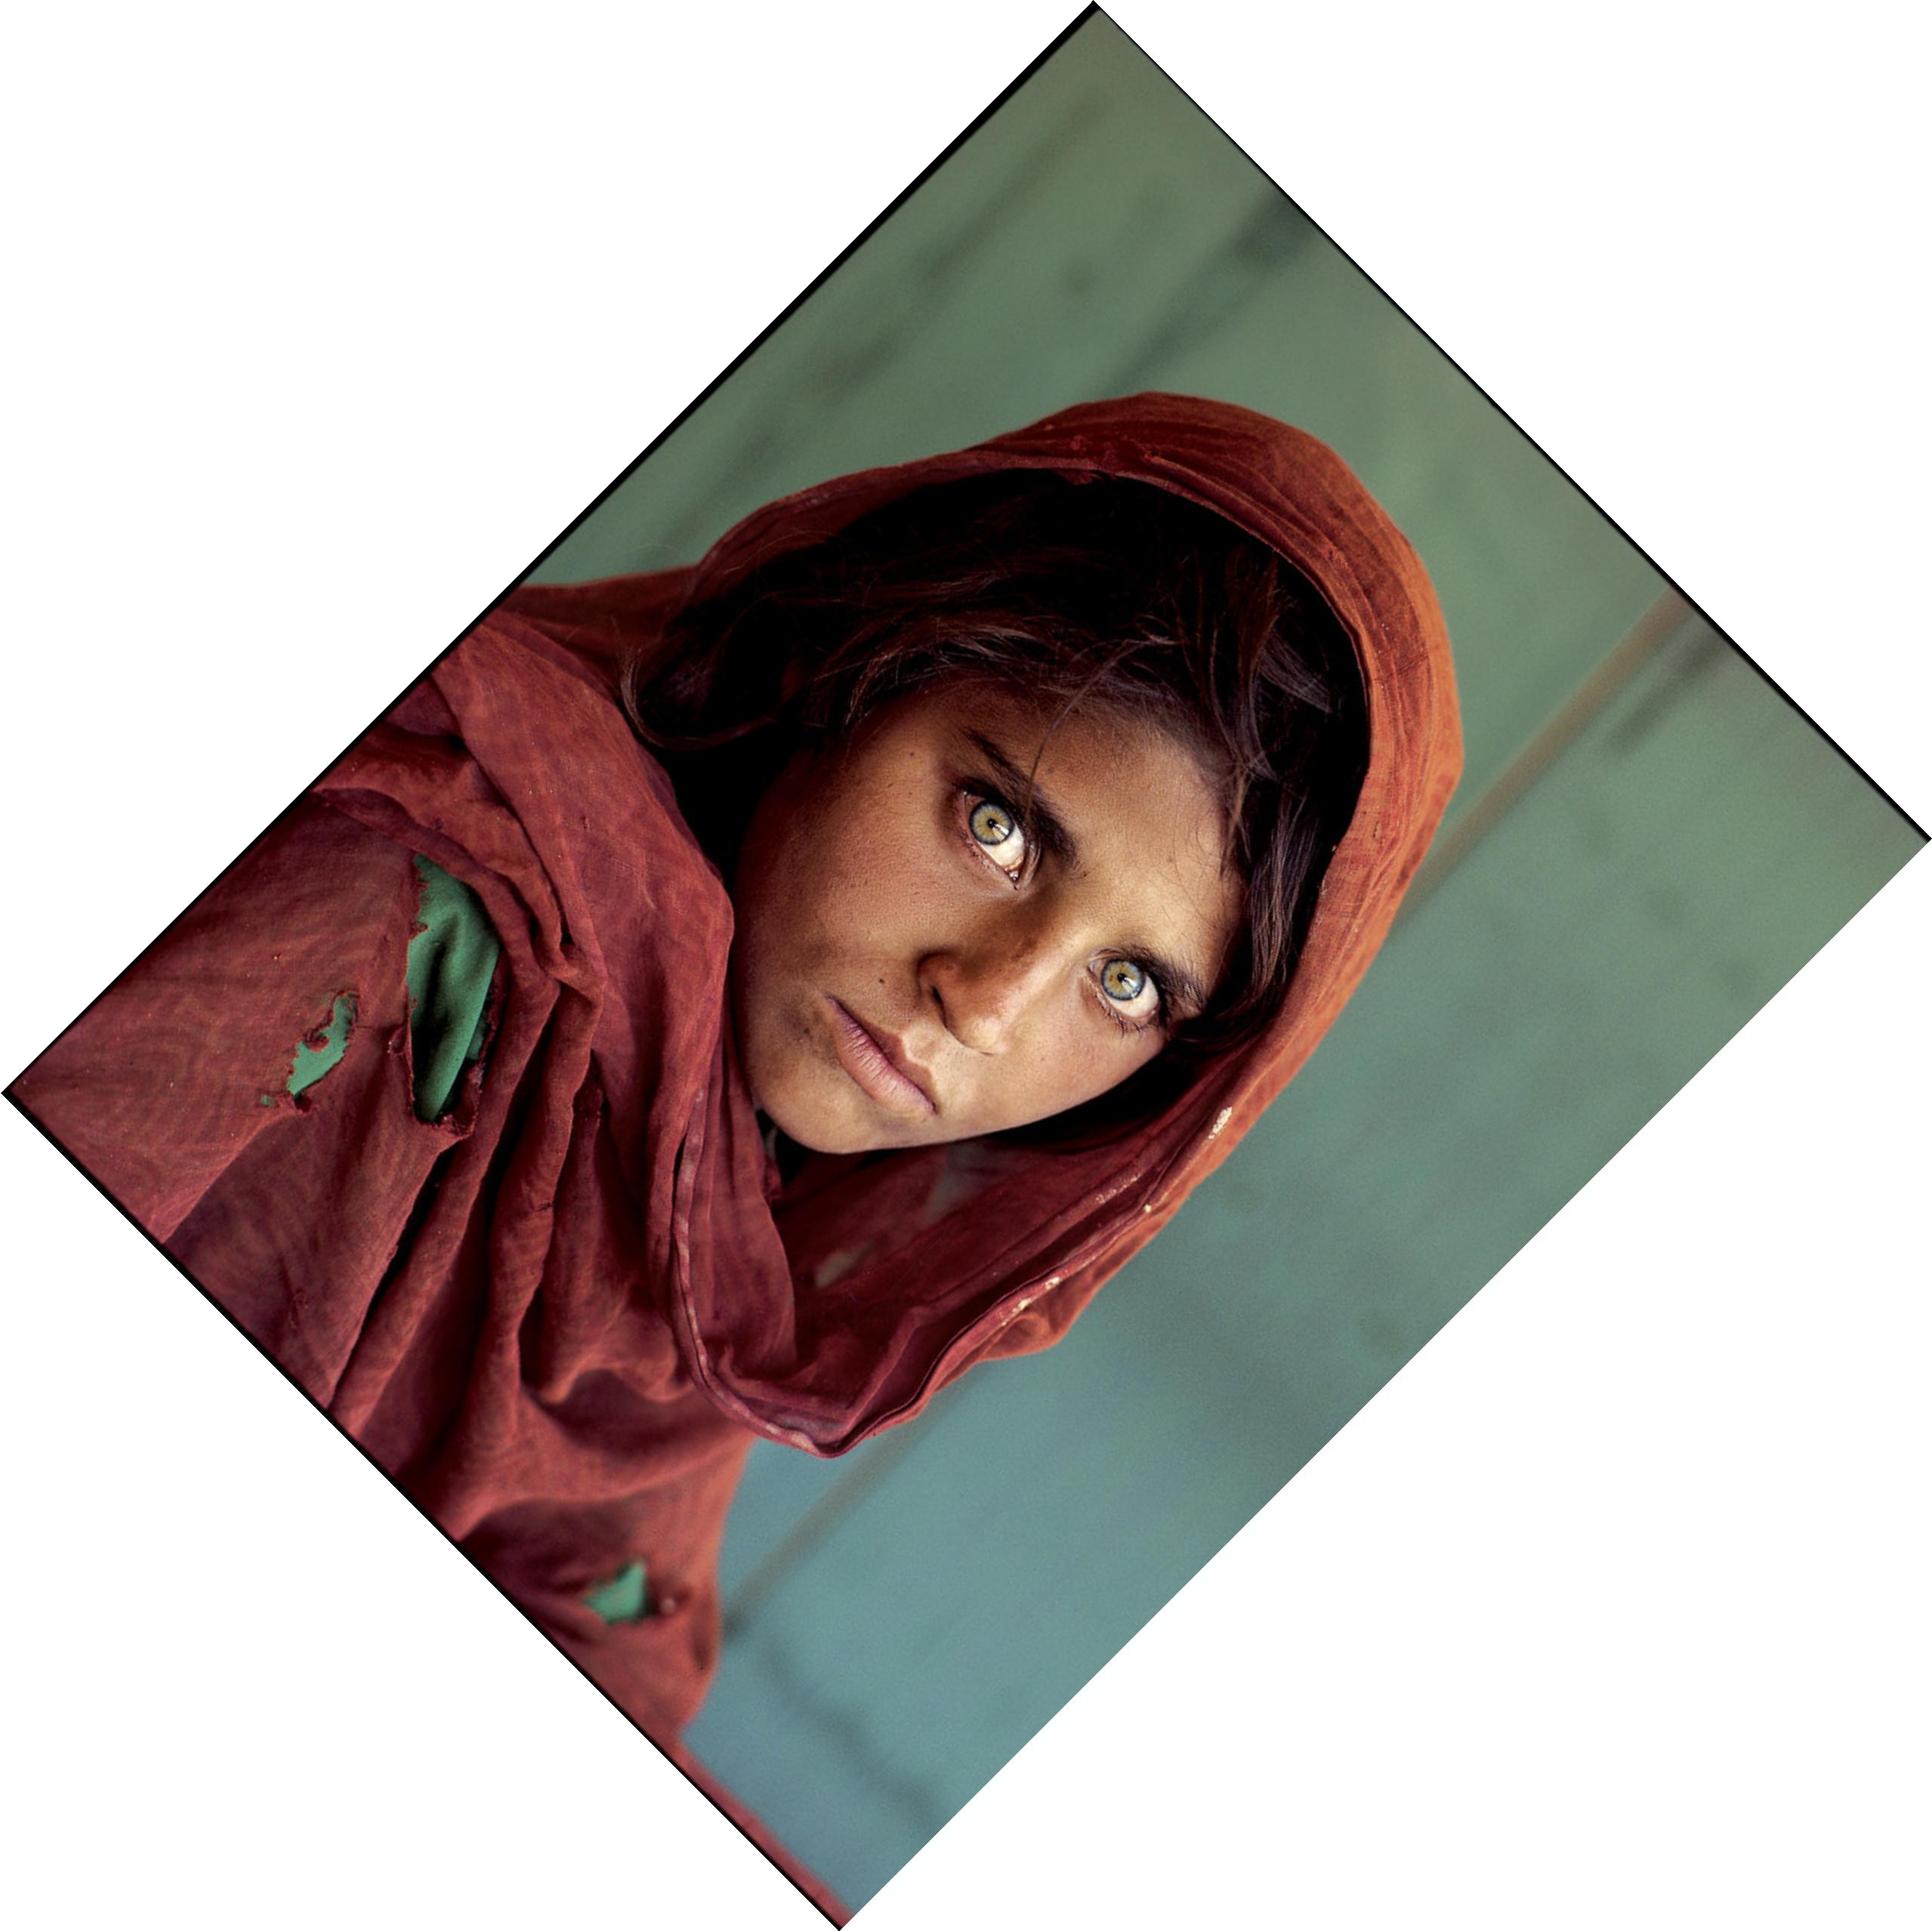
\includegraphics[scale=0.04]{q1/output/similar_2_1_2.jpg}
        \subcaption{}
    \end{subfigure}
    \begin{subfigure}{.3\textwidth}
        \centering
        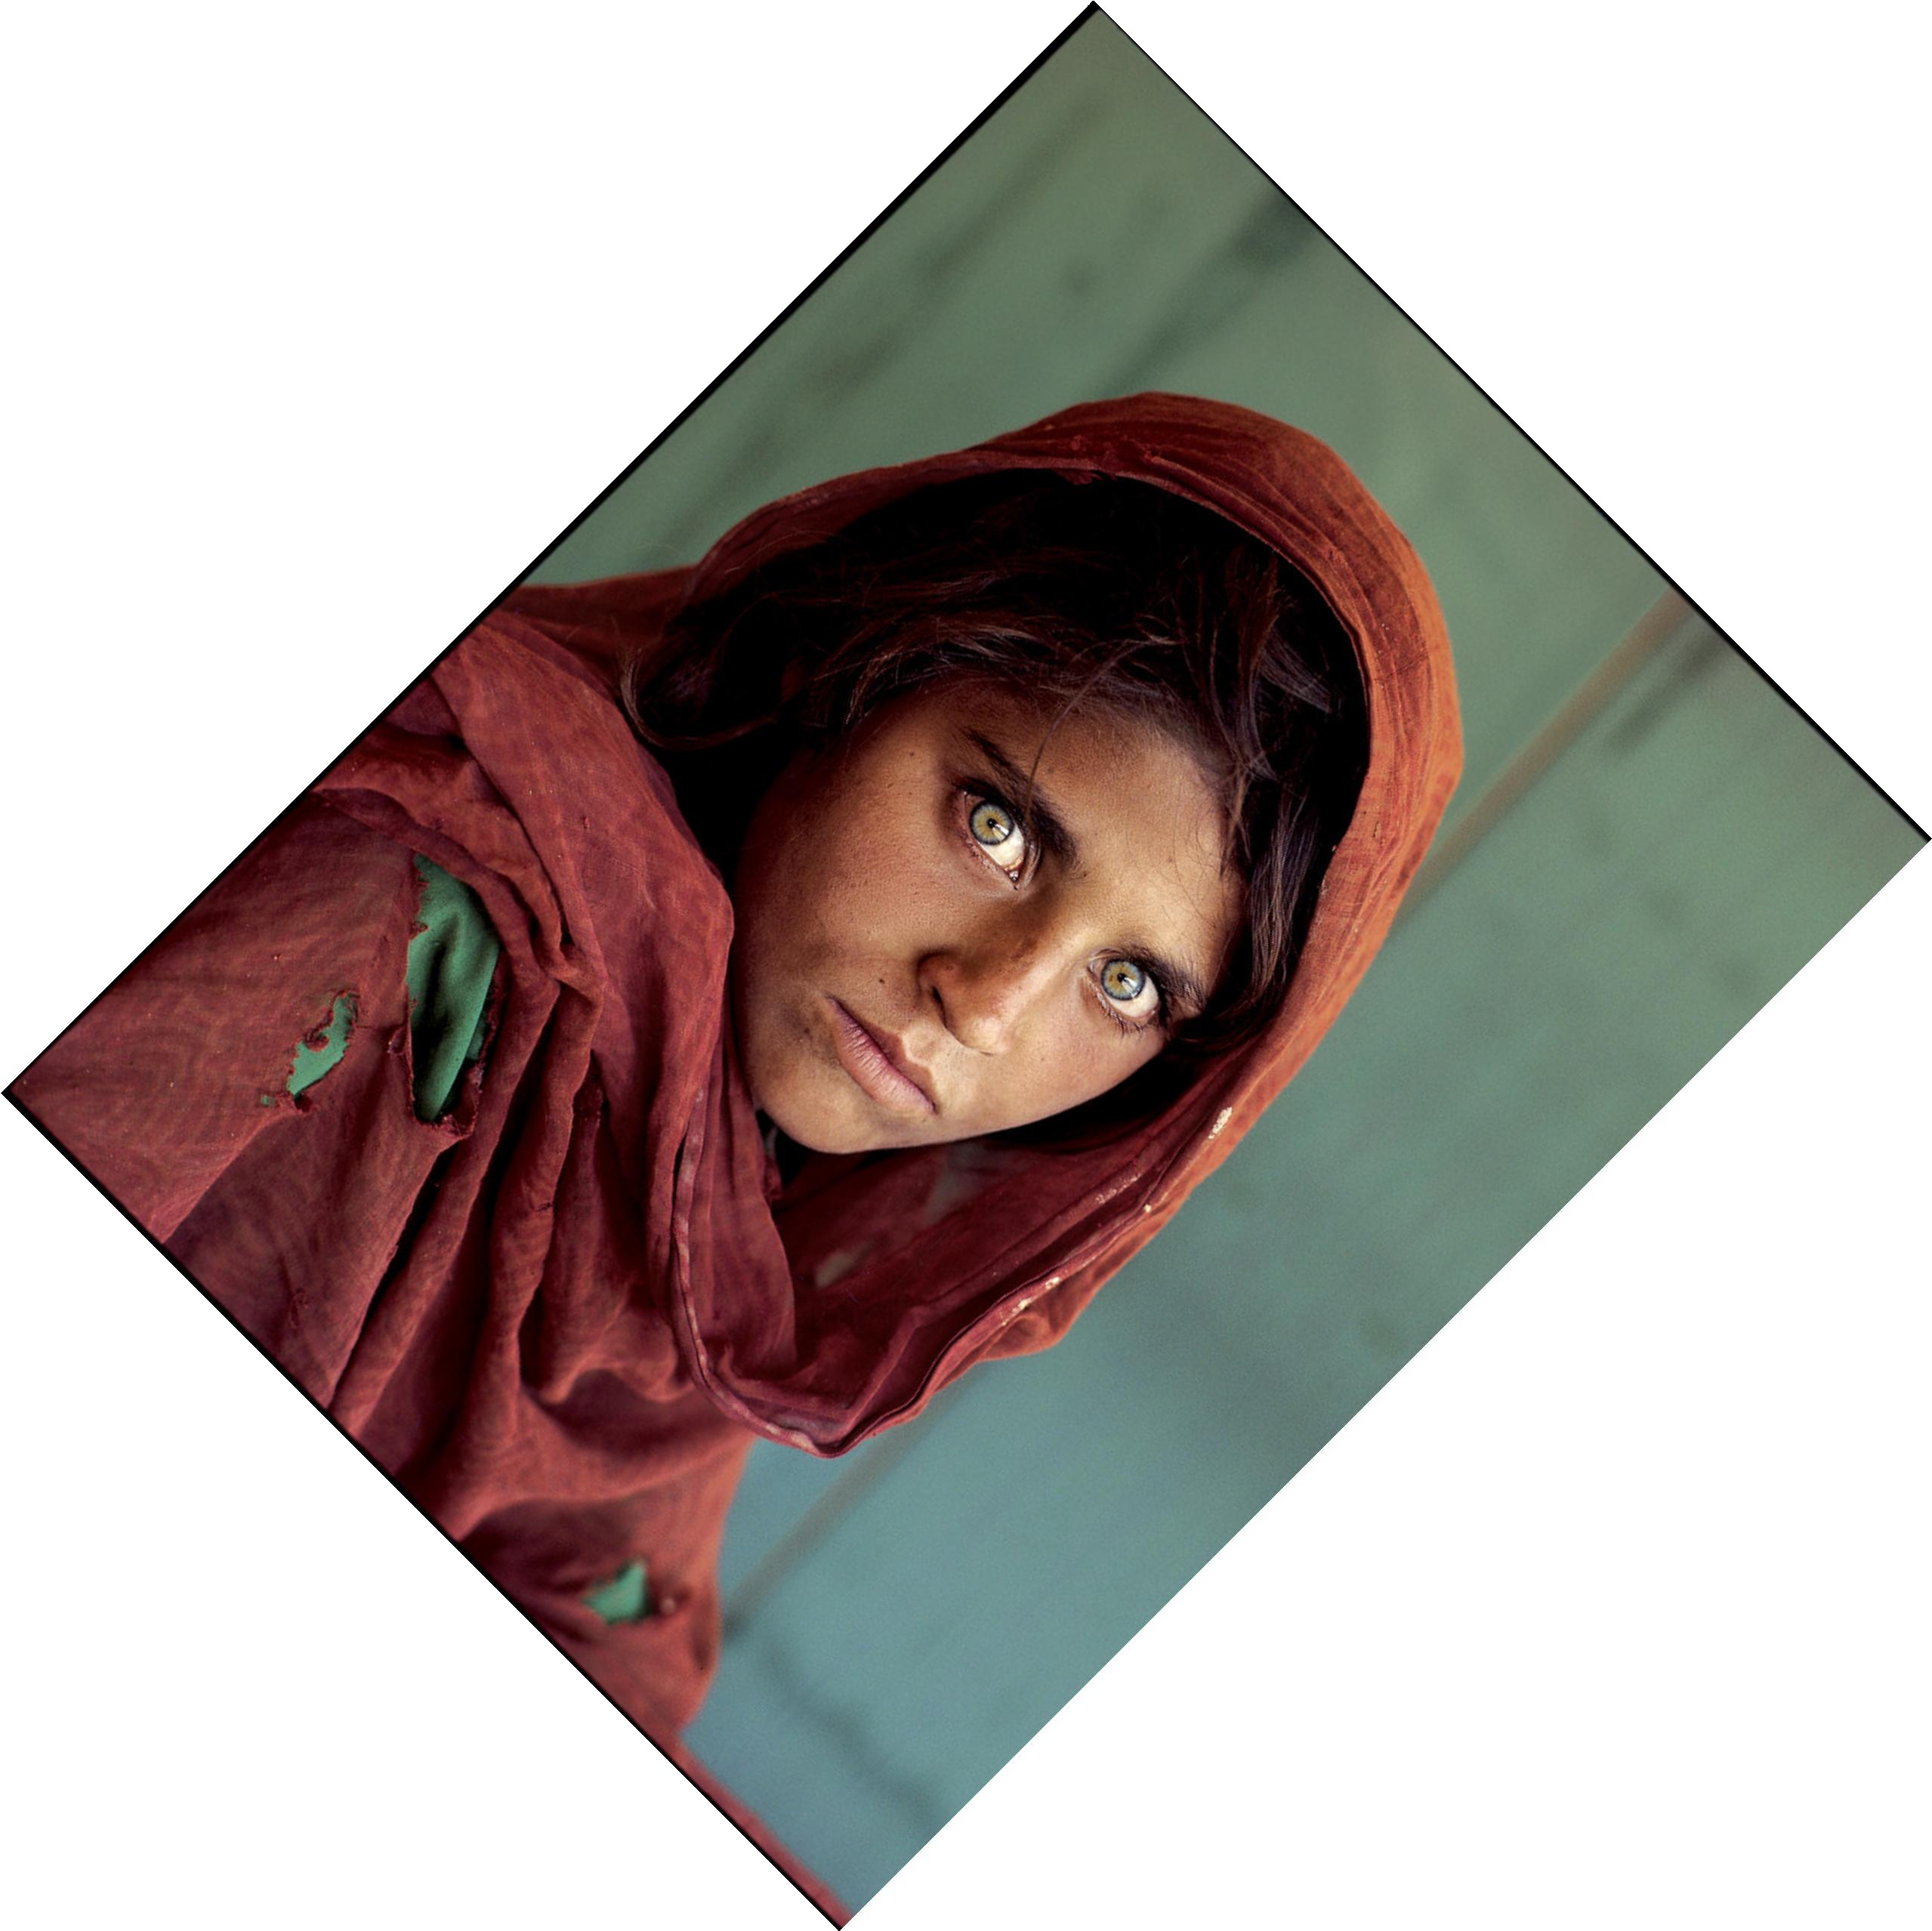
\includegraphics[scale=0.04]{q1/output/similar_2_2_2.jpg}
        \subcaption{}
    \end{subfigure}
    \caption{(a) blah (b) blah (c) blah}
\end{figure}

\subsection{Interpretation}
The \texttt{applyhomography.py} function is designed to compensate for the shift in the output image's origin. The code transforms the four corners of the input image using the homography matrix H. 
It then finds the minimum and maximum x and y coordinates. The size of the output image is then set to encompass all these points. 

\section{Question 2}
\begin{figure}[H]
    \centering
    \begin{subfigure}{.3\textwidth}
        \centering
        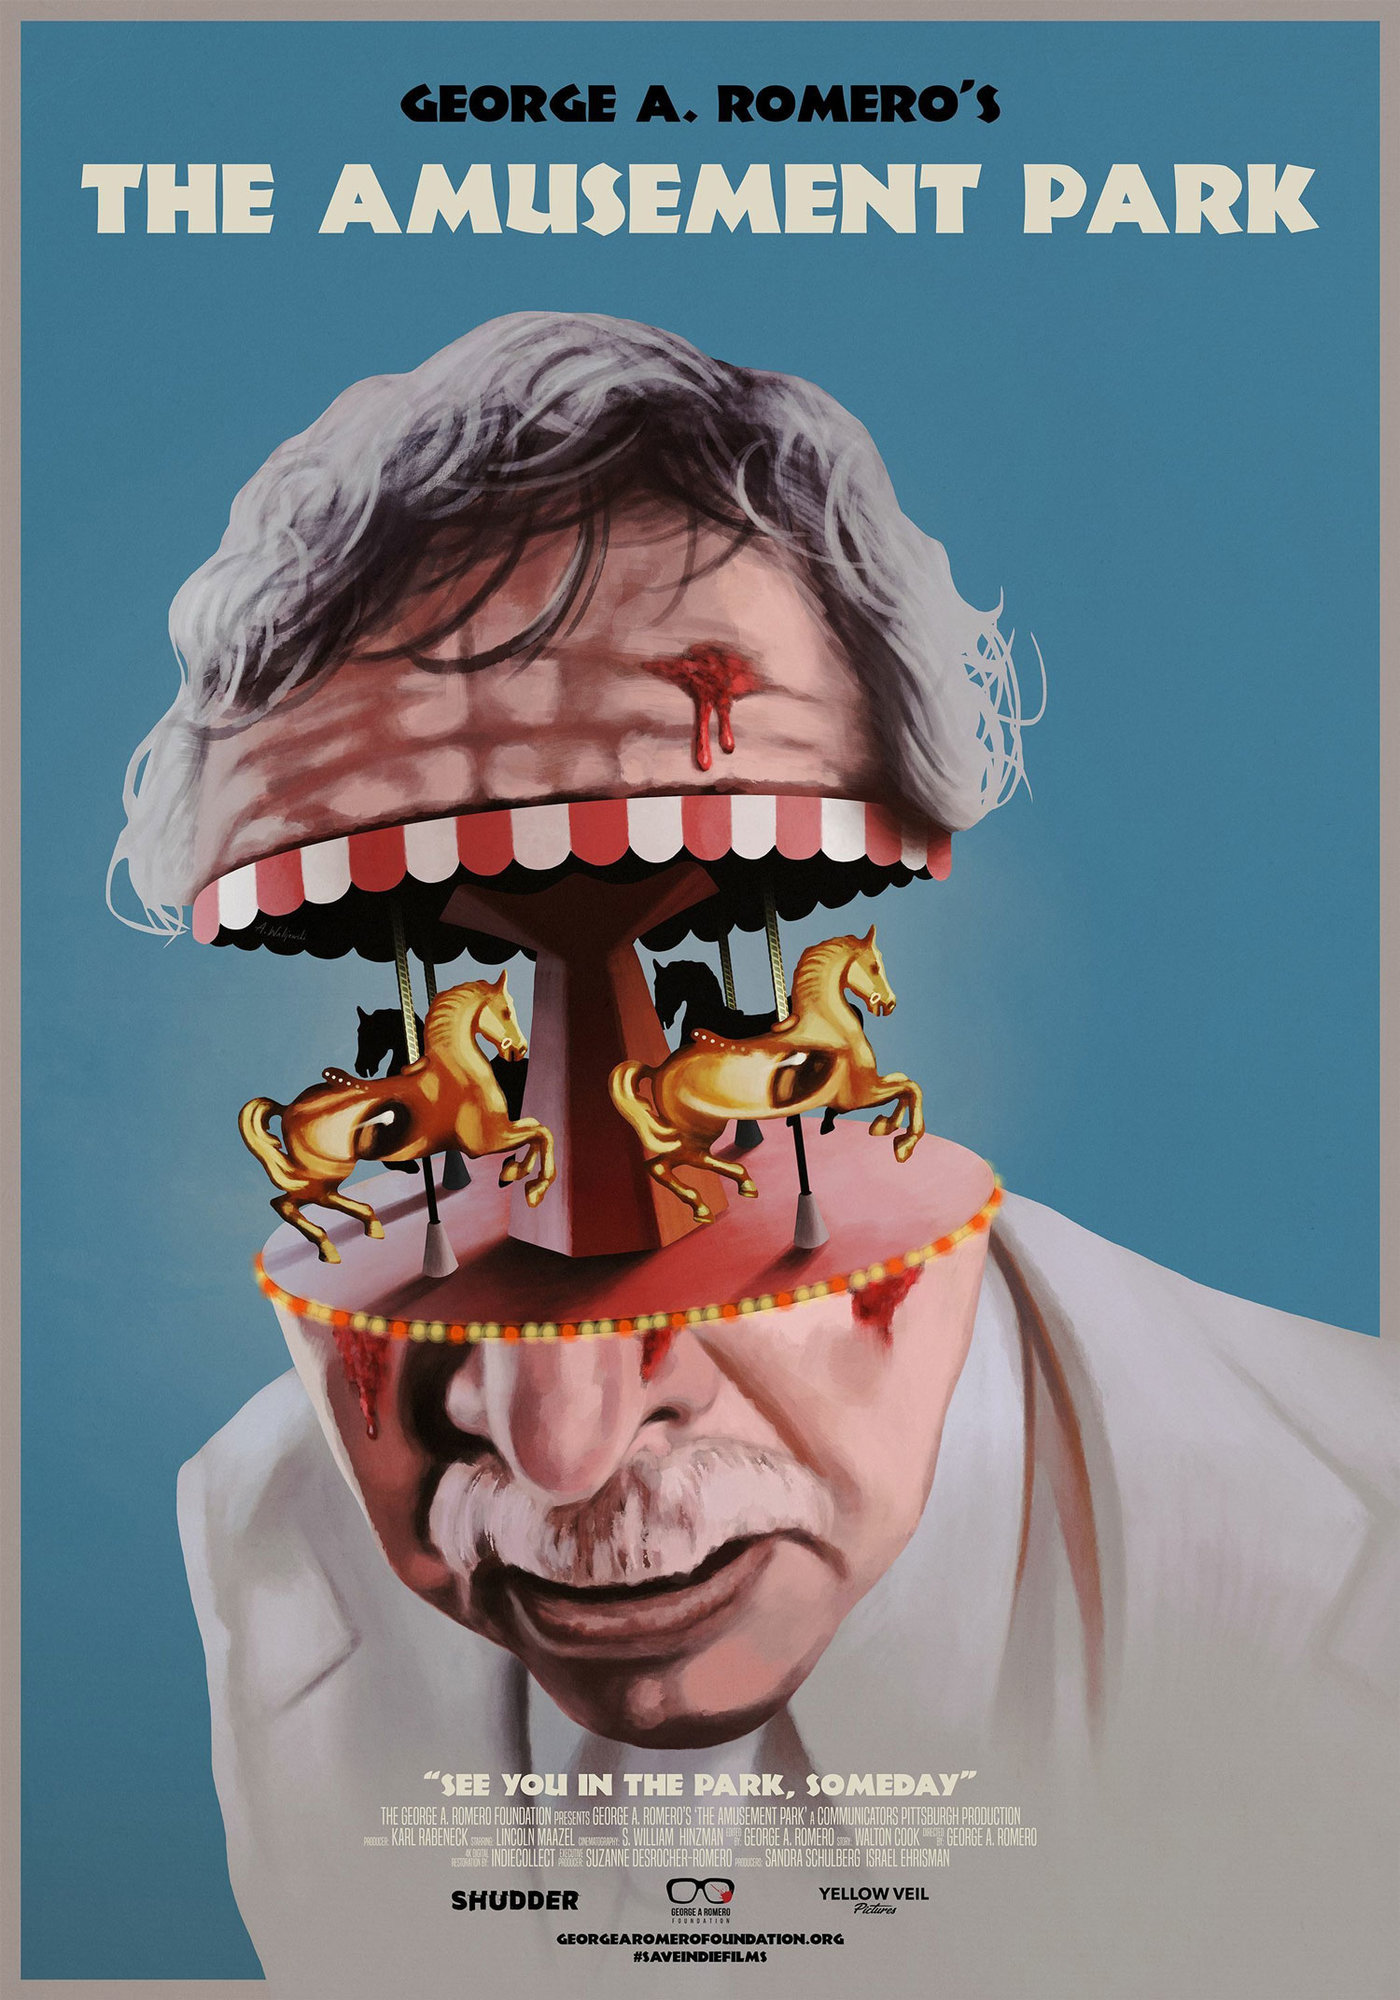
\includegraphics[scale=0.1]{q2/amuse.jpg}
        \subcaption{Original Movie Poster}
    \end{subfigure}
    \begin{subfigure}{.3\textwidth}
        \centering
        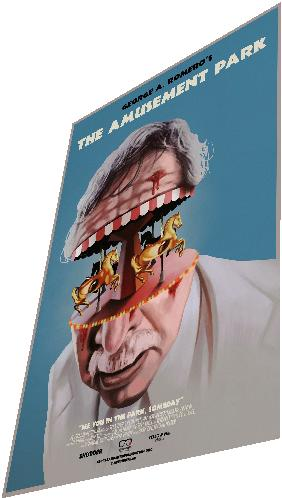
\includegraphics[scale=0.1]{q2/output/transform.jpg}
        \subcaption{Transformed Movie Poster}  
        \label{fig 1}
    \end{subfigure}
\end{figure}
\begin{figure}[H]
    \centering
    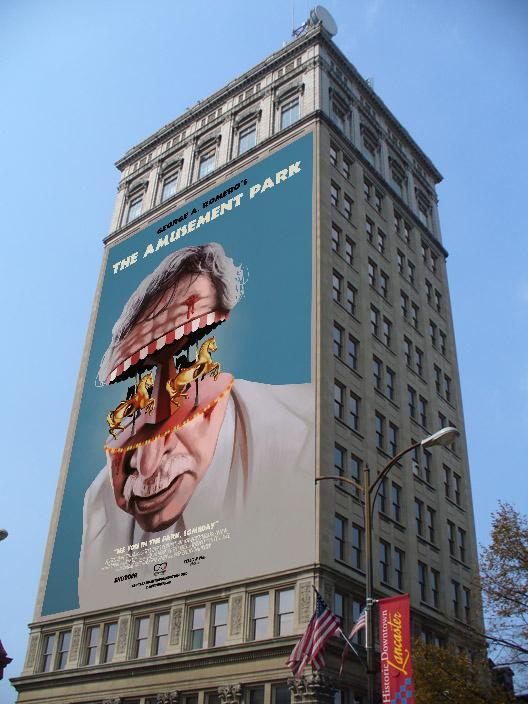
\includegraphics[scale=0.3]{q2/output/output.jpg}
    \caption{Building with Movie Poster}  
    \label{fig 2}
\end{figure}

\subsection{Interpretation}
\textbf{The transformed poster image will contain parts with no
image data that we want to ignore, and the image origin
may shift (why?). Explain how you addressed these two
issues.}
The transformed poster image contains a white region where there is no image data because the transformation maps some parts of the image
to areas that fall outside the original image bounds. To handle this, I created a mask: When pasting the transformed poster onto the building, 
the mask ensures that only the parts of the poster with actual content are pasted.

After applying the transformation, the origin of the poster shifts to a different position. This happens because the transformation can move the 
image in ways that push it outside the original image boundries. I compensate for this by calculating \texttt{minx} and \texttt{miny}. These
represent how much the image has shifted in the negative direction from the origin \texttt{(0,0)}. In this case, the minimum x and minimum y co-ordinates
shift by 35 and 124 units respectively. This offset ensures that the transformed poster aligns correctly with the intended location on the building image.

\textbf{Also, if we follow the interpolation procedure in the given code that applies homographies to images, it
turns out that our input (untransformed) poster image should be more-or-less similar in size to the desired
output (the transformed image). If the input is much larger, we get undesired “aliasing” artefacts in the
output. Experiment with this idea, and include in your report a short explanation of the issue of aliasing
in image interpolation.}
The original image is of size 1400 x 2000 and the building image is of size 528 x 704. 
\subsubsection{Case 1 : Large Input Image}
As one can observe in \ref{fig 1} and \ref{fig 2}. 
As one can observe, there are aliasing artifacts such as jagged edges and loss of fine detail. The downscaling process during the transformation 
fails to adequately capture the high frequency content. 

\subsubsection{Case 2 : Input Image of Same Size}
\begin{figure}[H]
    \centering
    \begin{subfigure}{.3\textwidth}
        \centering
        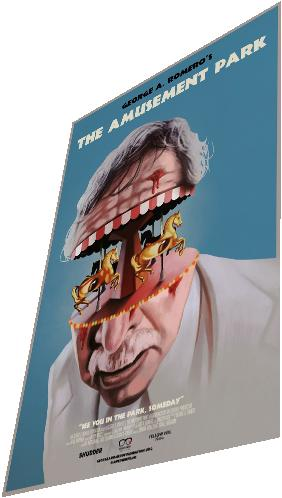
\includegraphics[scale=0.5]{q2/output/transform_same.jpg}
        \subcaption{Transformed Movie Poster}
    \end{subfigure}
    \begin{subfigure}{.3\textwidth}
        \centering
        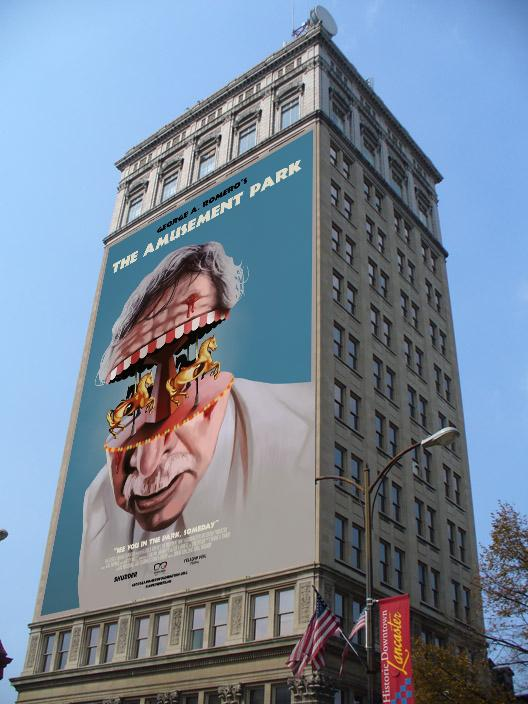
\includegraphics[scale=0.5]{q2/output/output_same.jpg}
        \subcaption{Building with Movie Poster}  
        \label{fig 1}
    \end{subfigure}
\end{figure}
The input image was changed to 528 x 704 to resemble the size of the output image. As one can observe, the image suffers from minimal aliasing. 

\subsubsection{Case 3 : Small Input Image}
\begin{figure}[H]
    \centering
    \begin{subfigure}{.3\textwidth}
        \centering
        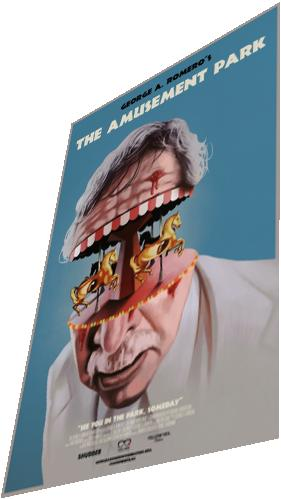
\includegraphics[scale=0.5]{q2/output/transform_small.jpg}
        \subcaption{Transformed Movie Poster}
    \end{subfigure}
    \begin{subfigure}{.3\textwidth}
        \centering
        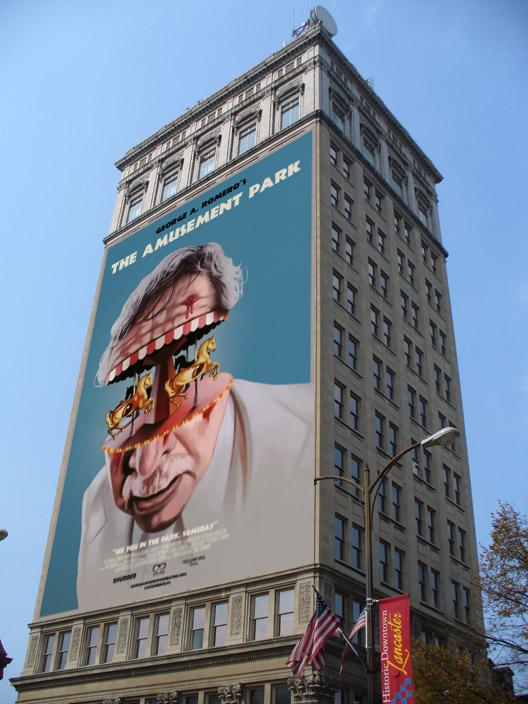
\includegraphics[scale=0.5]{q2/output/output_small.jpg}
        \subcaption{Building with Movie Poster}  
        \label{fig 1}
    \end{subfigure}
\end{figure}
The input image was now 250 x 350. The output poster is more blurred, but there are not as much aliasing artifacts as there were when the image 
was larger.  
\end{document}

